\scanpage{5}
\mspage{3}

premier. Comme application, Quillen obtient une interprétation faisceau\illegible{1}
que de la cohomologie d'un ensemble semi-simplicial à coéfficients dans \illegible{1}
système \begin{tabular}[b]{@{}l@{}}\inserted{\uline{local}}\\[-.65ex]\begin{tikzpicture}[x=1em,y=1em,baseline=0pt,line width=.45pt]\draw (2.8,.75) .. controls (3.1,.05) and (.4,-.05) .. (0,-.8);\end{tikzpicture}\end{tabular} con\deleted{tra}variant \begin{tabular}[b]{@{}l@{}}\inserted{$F$}\\[-.65ex]\begin{tikzpicture}[x=1em,y=1em,baseline=0pt,line width=.45pt]\draw (-.1,-.4)--(.8,.7);\end{tikzpicture}\end{tabular} d\deleted{\unsure{e}}(défini classiquement par le complexe cosimplici\unsure{a}
\margin{$\Pi$ ?} des $C^n(F) = \coprod_{x\unsure{\in|:}X_n} F(x)$ ): on considère le système local contravariant
défini par F, on l'interprète comme un faisceau sur \begin{tabular}[b]{@{}l@{}}\inserted{$T(X)$ i.e. objet de}\\[-.65ex]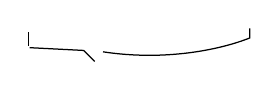
\begin{tikzpicture}[x=1em,y=1em,baseline=0pt,line width=.45pt]\draw (0,.25)--(0,-.25);\draw (.05,-.3)--(2,-.4)--(2.4,-.8);\draw (2.7,-.45) .. controls (5,-.8) and (7,-.35) .. (8,.05)--(8,.4);\end{tikzpicture}\end{tabular} $(\mathrm{Ssimpl})_{/X}$ , et on
prend sa cohomologie. - Cependant, quand F est un système de coéfficien\unsure{\deleted{s}t|\deleted{t}s}\illegible{1}
\margin{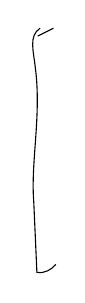
\begin{tikzpicture}[x=1mm,y=1mm]\draw (1,31) .. controls (-0.5,30) and (0.2,28) .. (0.4,26) .. controls (1.2,20) and (-0.2,14) .. (0.2,9) -- (0.6,0) .. controls (1.6,-0.2) and (2.5,0.4) .. (3,1); \draw (0.7,30) -- (2.7,31); \end{tikzpicture}}
covariant pas nécessairement local, on n'a tjrs pas d'interp\unsure{\deleted{é}r|\deleted{r}é}étation de \illegible{1}
\margin{Si !} groupes de cohomologie classiques en t ermes faiscdautiques; ni, lorsque
est \unsure{contravariant|contravatiant}, de son homologie, ou inversement de sa cohomologie
faisceautique en termes classiques.

A propos de la notion de foncteur qui est un homotopisme. Quillen
\margin{\begin{tikzpicture}[x=1mm,y=1mm]\draw[line width=.2pt] (0.5,30) -- (0.3,28); \draw[line width=.2pt,densely dashed] (0.3,28) .. controls (-0.1,20) and (0.1,7) .. (0.6,0); \draw[line width=.2pt,densely dashed] (1.2,19) -- (1.4,10); \draw[line width=.2pt] (1.4,10) -- (1.6,9.5) -- (2.3,9.4); \draw[line width=.2pt,densely dashed] (1.5,8.7) -- (2,0); \end{tikzpicture}}
montre qu\deleted{e}'un tel foncteur $F\colon C \to C'$ induit une équivalence entre la sou
catégorie triangulée \begin{tabular}[b]{@{}l@{}}\inserted{$D^b_{lc}(C')$}\\[-.65ex]\begin{tikzpicture}[x=1em,y=1em,baseline=0pt,line width=.45pt]\draw (0,-.7) .. controls (-.2,-.2) and (.15,.2) .. (.3,.05);\draw (.4,-.05)--(1.2,-.05);\draw (1.3,-.05) .. controls (3,.05) and (4.7,.5) .. (5,.85)--(4.9,1);\end{tikzpicture}\end{tabular} de la catégorie \inserted{dérivée \inserted{bornée} de celle \deleted{des}} des faisceaux abéliens sur C', don
les faisceaux de cohomologie sont des systèmes locaux, et la catégorie a\illegible{1}
logue pour C; \deleted{\unsure{Il s'en|Il en}} et réciproquement. \deleted{Pour la partie directe} On peut
dans cet énoncé introduire aussi n'importe quel anneau de base (à conditi
de le supposer $\neq 0$ dans le cas de la réciproque); \deleted{constant} la partie dir
vaut aussi avec un anneau de boefficients pas néc. constant, mais consta
tordu. Je pense que ce résultat (facile) doit pouvoir se généraliser ai
Soit $f\colon X \quad X'$ un morphisme de topos qui soit tel que pour tout \deleted{syst\unsure{è|ê}}
faisceau loc. const. sur X', f induise un isomorphisme sur les cohomolog
(avec cas non commutatif inclus). Supposons que \deleted{$\unsure{X|F}$ (resp. $\unsure{X|X'}$)} \inserted{\unsure{X} et X'} \unsure{\deleted{soi}t|soit} \uline{locale}
\margin{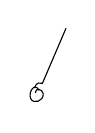
\begin{tikzpicture}[x=1mm,y=1mm]\draw (1.1,1.5) .. controls (0.5,2.6) and (-0.3,1.3) .. (0,0.5) .. controls (0.3,-0.3) and (1.7,0.1) .. (1.6,1.1) .. controls (1.5,1.7) and (0.6,1.9) .. (0.6,1.2); \draw (0.5,1.8) .. controls (0.8,2.7) and (1.2,2.4) .. (1.5,2.4) -- (4.5,9.4); \end{tikzpicture}}
\margin{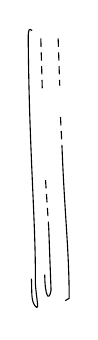
\begin{tikzpicture}[x=1mm,y=1mm]\draw (0.5,35) .. controls (0.1,35.3) and (0,35.2) .. (0,34) .. controls (0.1,20) and (1,10) .. (0.9,3) .. controls (1,1) and (1.5,-0.7) .. (0.9,0) .. controls (0.3,0.7) and (0.5,2) .. (0.4,3.5); \draw[densely dashed] (1.6,34) -- (1.8,27); \draw[densely dashed] (2.2,16) -- (2.6,10); \draw (2.6,10) -- (2.9,2) .. controls (2.6,0.4) and (2.1,1.5) .. (2.1,4); \draw[densely dashed] (3.8,34) -- (4,28); \draw[densely dashed] (4.1,24) -- (4.3,20); \draw (4.3,20) .. controls (4.6,12) and (5.2,7) .. (5.2,1) -- (4.7,0.7); \end{tikzpicture}}
\uline{homotopiquement trivial}, i.e. que \deleted{tout} pour tout entier n \begin{tabular}[b]{@{}l@{}}\inserted{$\geq 1$}\\[-.65ex]\begin{tikzpicture}[x=1em,y=1em,baseline=0pt,line width=.45pt]\draw (0,-.8) .. controls (.2,.1) and (1.6,.15) .. (1.8,.8)--(1.8,1);\end{tikzpicture}\end{tabular}, tout objet U \illegible{1}
\deleted{\unsure{X'|U'}} ait un \deleted{rev\unsure{ê}tement} \inserted{recouvrement} par des $U_i \to U$, tels que a) tout systême local sur
devient constant sur $U_i$ , et toute section sur U devient constante sur U
et b) pour tout \deleted{systême} groupe abélien G, les $H^j(U,G) \longrightarrow H^j(U_i,G)$ son
nuls pour $1 \leq j \leq n$. Alors le foncteur $D^b_{lc}(X') \longrightarrow D^b_{lc}(X)$ induit par f est

\noindent\begin{tikzpicture}[x=1cm,y=1cm,line width=0.3pt]
\draw (0,0)--(.08,.01);\draw (.12,.02) .. controls (.4,.06) and (.7,.04) .. (.9,.08)--(1.25,.12);\draw (1.29,.12)--(1.62,.15);\draw (1.67,.15)--(1.8,.16);\draw (1.84,.17)--(1.96,.18);\draw (2.1,.19)--(2.48,.22);\draw (2.53,.22)--(2.72,.23);\draw (2.78,.23)--(2.88,.23);\draw (3,.22) .. controls (3.3,.15) and (3.6,.14) .. (3.9,.13);\draw[densely dashed] (3.92,.13)--(4.35,.1);\draw (4.4,.1)--(4.75,.1);\draw[dotted] (5.9,.1)--(6.1,.1);\draw[densely dashed] (6.8,.06)--(7.1,.01);\draw[dotted] (7.15,.01)--(7.45,.02);\draw[densely dashed] (7.5,.03)--(7.9,.04);\draw[dotted] (7.95,.04)--(8.2,.05);\draw[densely dashed] (8.6,.07)--(8.95,.09);\draw[dotted] (9,.09)--(9.3,.1);\draw[densely dashed] (9.6,.12)--(10.2,.12);\draw[dotted] (10.25,.12)--(10.75,.11);\draw[densely dashed] (11.1,.11)--(11.6,.12);\draw (11.65,.12)--(11.83,.12);\draw[densely dashed] (11.88,.12)--(12.4,.12);\draw (12.45,.12)--(13.2,.1);
\end{tikzpicture}

\margin{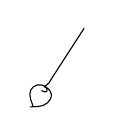
\begin{tikzpicture}[x=1mm,y=1mm]\draw (0.1,0).. controls (0.6,0.1) and (1.7,-0.1)..(2.3,0.5).. controls (3.3,1.4) and (2.7,2.2)..(2.2,2.5).. controls (1.4,3.1) and (0.5,2.8)..(0.2,2.1).. controls (-0.1,1.3) and (0.4,0.6)..(0.5,0.1); \draw (1.6,2.1).. controls (2.3,1.6) and (2.5,2.2)..(2.1,2.5); \draw (1.9,2.5).. controls (2.2,2.9) and (2.5,2.8)..(2.8,3.5) -- (7,10); \end{tikzpicture}}
\handwritten{Attention, cette condition n'est typiquement \uline{pas} satisfaite par les schémas a
leur \unsure{topologie} \unsure{étale} (mais bien \unsure{sur|par} \unsure{schémas|variétés} \unsure{l.}noeth. avec top. Zariski).}

\margin{4}
